% !TeX root = ../../main.tex
\section{工具总体结构设计}

多功能过滤工具\footnote{下文简称为“过滤工具”}是井筒高效清洁配套工具中的关键工具之一，由钻杆送入井下，在起钻过程中对井下钻井液进行过滤，分离并收集井底碎屑。其过滤功能独立于其他井下作业，不会影响正常下钻及循环。停泵上提过程中，该工具处于工作状态，扶正套筒移动并打开工具内部通道口，钻井液经工具内部的过滤外筒过滤后下行。

多功能过滤工具采用扶正套筒开关设计：下入时，扶正套筒关闭工具内部通道口，不影响工具串正常下钻及作业；上提时，扶正套筒打开工具内部通道口，过滤工具开始工作。

多功能过滤工具设置有观察孔及清理盖板：观察孔便于检查碎屑的收集量；清理盖板在工具作业完成后即可拆卸，以清理储存的碎屑，无需拆卸工具本体。

多功能过滤工具的结构如图~\ref{fig:filter_tool_structure}所示，主要由提升短节、上扶正套筒、扶正块、滤进接头、过滤套筒、过滤外筒、过滤内筒、清理盖板、滤出接头、下扶正套筒和下接头组成。其中，过滤套筒、过滤外筒和过滤内筒可替换为加长版，以增大过滤容量。

其工作原理为：工具下井后，扶正套筒受力上行，关闭工具内部通道口，此时过滤工具不工作，工具串可进行正常作业；当工具串上提时，扶正套筒受力下行，打开工具内部通道口，过滤工具开始工作。带有碎屑的钻井液进入工具内部，由过滤外筒完成过滤，经过滤内筒循环回井内。

\begin{figure}[htbp]
  \centering % 图片居中
  \includegraphics[width=1.0\textwidth]{figure/chapter3/guolvqi.png} % 图片路径
  \caption{多功能过滤工具结构示意图} % 图标题
  \label{fig:filter_tool_structure} % 标签，用于文中引用
\end{figure}

过滤工具的主要技术参数见表~\ref{tab:filter_tool_params}。

\begin{table}[htbp]
    \centering
    \caption{多功能过滤工具技术参数表}
    \label{tab:filter_tool_params}
    \footnotesize % 共 11 列，缩小字号以适应宽表格
    \setlength{\tabcolsep}{3pt} % 减小列间距，避免超出正文版心
    \renewcommand{\arraystretch}{1.3} % 增加行高
    
    \begin{tabularx}{\textwidth}{Xcccccccccc}
        \toprule
        型号 & 
        \begin{tabular}[c]{@{}c@{}}适用\\套管\\(in)\end{tabular} & 
        上部扣型 & 
        下部扣型 & 
        \begin{tabular}[c]{@{}c@{}}长度\\(mm)\end{tabular}& 
        \begin{tabular}[c]{@{}c@{}}本体\\外径\\(mm)\end{tabular}& 
        \begin{tabular}[c]{@{}c@{}}本体\\内径\\(mm)\end{tabular}& 
        \begin{tabular}[c]{@{}c@{}}许用抗拉\\强度\\(kN)\end{tabular}& 
        \begin{tabular}[c]{@{}c@{}}许用抗扭\\强度\\($\text{kN}\cdot\text{m}$)\end{tabular} & 
        \begin{tabular}[c]{@{}c@{}}最大\\转数\\(rpm)\end{tabular} & 
        \begin{tabular}[c]{@{}c@{}}碎屑存储量\\(L)\end{tabular} \\
        \midrule
        
        GLGJ70000A & 7 & NC38 & NC38 & 6500 & 139.7 & 35.06 & 2500 & 39 & 120 & 6.90 \\
        
        \midrule
        
        \begin{tabular}[c]{@{}c@{}}GLGJ70000A-\\加长版\end{tabular} & 7 & NC38 & NC38 & 8786.24 & 139.7 & 35.06 & 2500 & 39 & 120 & 15.85 \\
        \bottomrule
    \end{tabularx}
\end{table}


\section[过滤工具设计计算与校核]{过滤工具设计计算与校核\protect\footnote{合同条款：5.2.1.3井筒高效清洁关键技术配套工具设计——（3）多功能过滤工具：工作允许旋转$>=120\text{rpm}$，工具内通径$>=2.688\inch$，碎屑存储量$>=30\textrm{L}$}}


\subsection{主要受力件的螺纹强度校核}

过滤工具的主要受力件为提升短节、滤进接头、滤出接头和下接头，其连接螺纹均为 3.625\inch-8 Stub ACME（材料 4145H）。

螺纹牙的剪切强度按下式计算：
\begin{align}
    F_{\max} &= [\tau] \cdot k_z \cdot \pi \cdot d_1 \cdot b \cdot z \cdot 10^{-3} \\
    [\tau] &= \frac{\sigma_s}{n}
\end{align}
式中，$F_{\max}$---工具最大拉力，kN；

$[\tau]$---螺纹牙的许用剪切强度，MPa；

$k_z$---螺纹各圈的载荷不均系数，根据《机械设计手册》螺纹连接（紧固件连接）部分中螺纹牙的剪切强度计算及各圈螺纹载荷分配的规定\cite{ref26}，取 $k_z = 0.56$；

$d_1$---螺纹底径，mm；

$b$---螺纹牙根宽度，mm；

$z$---旋合圈数；

$\sigma_s$---材料最小屈服强度，取 930 MPa；

$n$---安全系数，根据《机械设计手册》螺纹连接部分中螺纹牙强度校核的安全系数取值规定\cite{ref26}，取 $n = 2.5$。

将 3.625\inch-8 Stub ACME 螺纹的相关参数代入，计算得：
\begin{align}
    F_{\max} &= [\tau] \cdot k_z \cdot \pi \cdot d_1 \cdot b \cdot z \cdot 10^{-3} \\
             &= 372 \times 0.56 \times 3.14 \times 89.66 \times 1.310 \times 22 \times 10^{-3} \\
             &= 1690.26\,\text{kN} \\
             &> 1000\,\text{kN}
\end{align}

计算结果表明，螺纹牙的剪切强度满足设计要求。


\subsection{主要受力件的零件抗拉强度校核}

过滤工具的主要受力件为提升短节、滤进接头、滤出接头和下接头，各受力件的抗拉危险截面为：

提升短节：3.625\inch-8 Stub ACME 内螺纹根部；

滤进接头：3.625\inch-8 Stub ACME 外螺纹根部与凹槽根部；

滤出接头：3.625\inch-8 Stub ACME 外螺纹根部与凹槽根部；

下接头：3.625\inch-8 Stub ACME 内螺纹根部。

抗拉强度按下式计算：
\begin{equation}
F_{\max} = \frac{\pi \cdot (D^2 - d^2) \cdot \sigma_s}{4 \cdot n} \times 10^{-3}
\end{equation}
式中，$F_{\max}$---工具最大拉力，kN；

$D$---危险截面外径，mm；

$d$---危险截面内径，mm；

$\sigma_s$---材料最小屈服强度，取 930 MPa；

$n$---安全系数，取 $n = 1.5$。

（1）提升短节 3.625\inch-8 Stub ACME 内螺纹根部最大拉力
\begin{align}
    F_{\max} &= \frac{\pi \cdot (D^2 - d^2) \cdot \sigma_s}{4 \cdot n} \times 10^{-3} 
             = \frac{3.14 \times (120.65^2 - 93.40^2) \times 930}{4 \times 1.5} \times 10^{-3} \\
             &= 2838.85\,\text{kN} > 1000\,\text{kN}
\end{align}
满足设计要求。

（2）滤进接头 3.625\inch-8 Stub ACME 外螺纹根部最大拉力
\begin{align}
    F_{\max} &= \frac{\pi \cdot (D^2 - d^2) \cdot \sigma_s}{4 \cdot n} \times 10^{-3} 
             = \frac{3.14 \times (88.09^2 - 45.72^2) \times 930}{4 \times 1.5} \times 10^{-3} \\
             &= 2759.36\,\text{kN} > 1000\,\text{kN}
\end{align}
满足设计要求。

（3）滤进接头凹槽根部最大拉力（该处截面不规则，面积由实体测量得到）
\begin{equation}
F_{\max} = \frac{A \cdot \sigma_s}{n} \times 10^{-3} = \frac{3523.3 \times 930}{1.5} \times 10^{-3} = 2184.4\,\text{kN} \geq 1000\,\text{kN}
\end{equation}
满足设计要求。

（4）滤出接头 3.625\inch-8 Stub ACME 外螺纹根部最大拉力
\begin{align}
    F_{\max} &= \frac{\pi \cdot (D^2 - d^2) \cdot \sigma_s}{4 \cdot n} \times 10^{-3} 
             = \frac{3.14 \times (88.60^2 - 44.45^2) \times 930}{4 \times 1.5} \times 10^{-3} \\
             &= 2858.95\,\text{kN} > 1000\,\text{kN}
\end{align}
满足设计要求。

（5）滤出接头凹槽根部最大拉力（该处截面不规则，面积由实体测量得到）
\begin{equation}
F_{\max} = \frac{A \cdot \sigma_s}{n} \times 10^{-3} = \frac{3185.38 \times 930}{1.5} \times 10^{-3} = 1974.94\,\text{kN} \geq 1000\,\text{kN}
\end{equation}
满足设计要求。

（6）下接头 3.625\inch-8 Stub ACME 内螺纹根部最大拉力
\begin{align}
    F_{\max} &= \frac{\pi \cdot (D^2 - d^2) \cdot \sigma_s}{4 \cdot n} \times 10^{-3} 
             = \frac{3.14 \times (120.65^2 - 93.40^2) \times 930}{4 \times 1.5} \times 10^{-3} \\
             &= 2838.85\,\text{kN} > 1000\,\text{kN}
\end{align}
满足设计要求。


\subsection{主要受力件的零件抗扭强度校核}

过滤工具的主要受力件为提升短节、滤进接头、滤出接头和下接头，各受力件的抗扭危险截面为：

提升短节：3.625\inch-8 Stub ACME 内螺纹根部；

滤进接头：3.625\inch-8 Stub ACME 外螺纹根部；

滤出接头：3.625\inch-8 Stub ACME 外螺纹根部；

下接头：3.625\inch-8 Stub ACME 内螺纹根部。

抗扭强度按下式计算：
\begin{align*}
    \tau &= \frac{16 \cdot D \cdot T_{\max}}{\pi \cdot (D^4 - d^4)} \times 10^{6} \\
    T_{\max} &= \frac{[\tau] \cdot \pi \cdot (D^4 - d^4)}{16 \cdot D} \times 10^{-6} \\
    [\tau] &= n \cdot \sigma_s = 0.66 \times 930\,\text{MPa} = 620\,\text{MPa}
\end{align*}
式中，$T_{\max}$---工具最大扭矩，$\text{kN} \cdot \text{m}$；

$\tau$---危险截面的切应力，MPa；

$[\tau]$---材料许用切应力，MPa；

$\sigma_s$---材料屈服强度，MPa；

$D$---危险截面外径，mm；

$d$---危险截面内径，mm；

$n$---许用切应力与许用拉应力之比，根据《机械设计手册》零件强度校核中许用应力折减系数的取值规定\cite{ref26}，取 $n=0.66$。

（1）提升短节 3.625\inch-8 Stub ACME 内螺纹根部最大扭矩
\begin{align}
    T_{\max} &= \frac{[\tau] \cdot \pi \cdot (D^4 - d^4)}{16 \cdot D} \times 10^{-6} 
             = \frac{620 \times 3.14 \times (120.65^4 - 45.72^4)}{16 \times 120.65} \times 10^{-6} \\
             &= 209.28\,\text{kN} \cdot \text{m} > 18\,\text{kN} \cdot \text{m}
\end{align}
满足设计要求。

（2）滤进接头 3.625\inch-8 Stub ACME 外螺纹根部最大扭矩
\begin{align}
    T_{\max} &= \frac{[\tau] \cdot \pi \cdot (D^4 - d^4)}{16 \cdot D} \times 10^{-6} 
             = \frac{620 \times 3.14 \times (88.09^4 - 45.72^4)}{16 \times 88.09} \times 10^{-6} \\
             &= 77.14\,\text{kN} \cdot \text{m} > 18\,\text{kN} \cdot \text{m}
\end{align}
满足设计要求。

（3）滤出接头 3.625\inch-8 Stub ACME 外螺纹根部最大扭矩
\begin{align}
    T_{\max} &= \frac{[\tau] \cdot \pi \cdot (D^4 - d^4)}{16 \cdot D} \times 10^{-6} 
             = \frac{620 \times 3.14 \times (88.60^4 - 44.45^4)}{16 \times 88.60} \times 10^{-6} \\
             &= 79.26\,\text{kN} \cdot \text{m} > 18\,\text{kN} \cdot \text{m}
\end{align}
满足设计要求。

（4）下接头 3.625\inch-8 Stub ACME 内螺纹根部最大扭矩
\begin{align}
    T_{\max} &= \frac{[\tau] \cdot \pi \cdot (D^4 - d^4)}{16 \cdot D} \times 10^{-6} 
             = \frac{620 \times 3.14 \times (120.65^4 - 93.40^4)}{16 \times 120.65} \times 10^{-6} \\
             &= 136.94\,\text{kN} \cdot \text{m} > 18\,\text{kN} \cdot \text{m}
\end{align}
满足设计要求。


在上述理论计算的基础上，采用有限元方法对主要受力件的结构强度进行复核。过滤工具的薄弱零件及其受载后的应力分布分别如图~\ref{fig:weak_part_filter}和图~\ref{fig:weak_part_filter_fea}所示，主要受力件为提升短节、下接头、滤进接头和滤出接头，危险截面出现在螺纹根部及变径处。

滤出接头的最大拉应力为 238 MPa，远小于设计要求；最大切应力为 2555 MPa，出现在变径处，但范围极小，属于应力集中导致的局部小尺度高应力，不会引发整体塑性变形，强度满足设计要求。滤进接头的最大拉应力为 206 MPa，远小于设计要求；最大切应力为 2610 MPa，出现在变径处，但范围极小，属于应力集中导致的局部小尺度高应力，不会引发整体塑性变形，强度满足设计要求。

\begin{figure}[htbp]
    \centering
    % 子图 (a)
    \subfloat[滤出接头]{%
        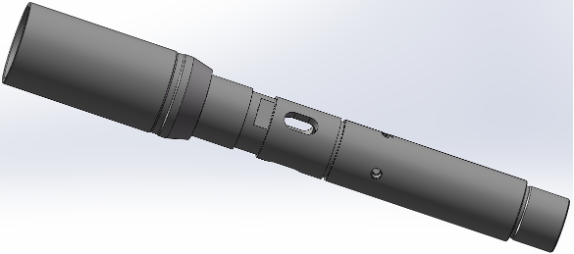
\includegraphics[width=0.4\linewidth]{figure/chapter3/filter-outlet-sub.png}%
        \label{fig:filter_outlet_sub}
    }
    %\hfill
    % 子图 (b)
    \subfloat[滤进接头]{%
        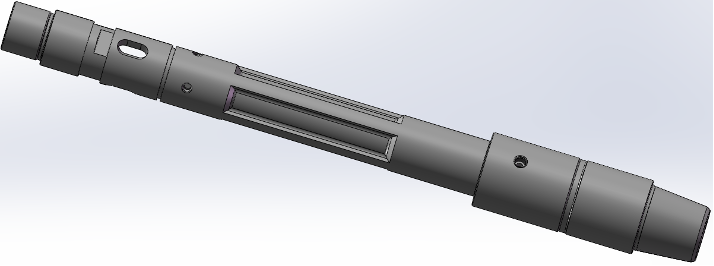
\includegraphics[width=0.5\linewidth]{figure/chapter3/filter-inlet-sub.png}%
        \label{fig:filter_inlet_sub}%
    }
        \caption{过滤工具薄弱零件}
    \label{fig:weak_part_filter}
\end{figure}


\begin{figure}[htbp]
    \centering
    % 子图 (a)
    \subfloat[滤出接头受拉应力分布]{%
        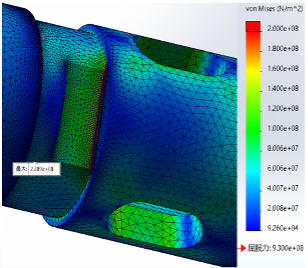
\includegraphics[width=0.45\linewidth]{figure/chapter3/filter-outlet-sub-tensile-stress.png}%
        \label{fig:fea_filter_outlet_tension}
    }
    \hfill
    % 子图 (b)
    \subfloat[滤出接头受扭应力分布]{%
        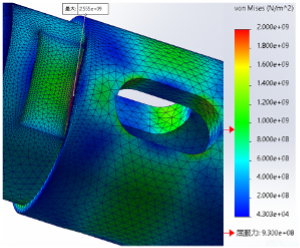
\includegraphics[width=0.45\linewidth]{figure/chapter3/filter-outlet-sub-torsion-stress.png}%
        \label{fig:fea_filter_outlet_torsion}
    }
    \vspace{1em}
      % 子图 (c)
    \subfloat[滤进接头受拉应力分布]{%
        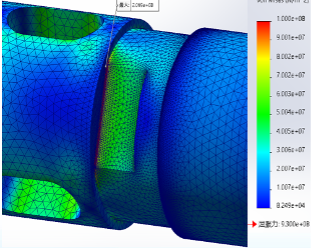
\includegraphics[width=0.45\linewidth]{figure/chapter3/filter-inlet-sub-tensile-stress.png}%
        \label{fig:fea_filter_inlet_tension}
    }
    \hfill
      % 子图 (d)
    \subfloat[滤进接头受扭应力分布]{%
        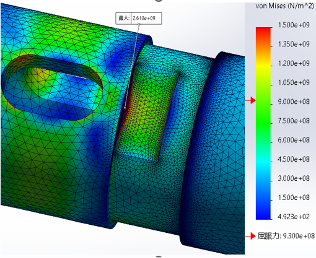
\includegraphics[width=0.45\linewidth]{figure/chapter3/filter-inlet-sub-torsional-stress.png}%
        \label{fig:fea_filter_inlet_torsion}
    }
        \caption{过滤工具薄弱零件受载有限元分析结果}
    \label{fig:weak_part_filter_fea}
\end{figure}


\subsection{过滤容积计算}

过滤工具容量 $V$ 的计算式为：
\begin{equation}
V = L \cdot A = L \cdot \frac{\pi \cdot (D^2 - d^2)}{4} \times 10^{-6}
\end{equation}
式中，$V$---过滤容量，L；

$L$---过滤腔长度，mm；

$A$---过滤腔环形截面积，$\text{mm}^2$；

$D$---大径，mm；

$d$---小径，mm。

代入数值计算得：
\begin{align}
    V &= L \cdot A = L \cdot \frac{\pi \cdot (D^2 - d^2)}{4} \times 10^{-6} \\
      &= 4864.56 \times \frac{\pi \cdot (100.26^2 - 73.03^2)}{4} \times 10^{-6} \\
      &= 18.0\,\text{L} \ge 15\,\text{L}
\end{align}
满足设计要求。

各主要受力件的强度校核结果汇总见表~\ref{tab:force_data_filter}。

\begin{table}[htbp]
    \centering
    \caption{受力件数据统计表}
    \label{tab:force_data_filter}
    \renewcommand{\arraystretch}{1.5} % 增加行高，使表格更美观
    \begin{tabularx}{.9\textwidth}{Xc}
        \toprule % 顶线
        \textbf{受力类型} & \textbf{数据} \\
        \midrule % 栏目线
        材料屈服强度 $\sigma_s$ & $930\,\text{MPa}$ \\
        螺纹最大剪切力 $F_{\max1}$ & $1690.3\,\text{kN}$ \\
        提升短节最大拉力 $F_{\max2}$ & $2838.8\,\text{kN}$ \\
        滤进接头最大拉力 $F_{\max3}$ & $2759.4\,\text{kN}$ \\
        滤出接头最大拉力 $F_{\max4}$ & $2859.0\,\text{kN}$ \\
        下接头最大拉力 $F_{\max5}$ & $2838.8\,\text{kN}$ \\
        材料许用切应力 $[\tau]$ & $620\,\text{MPa}$ \\
        最大扭矩 & $39\,\text{kN}\cdot\text{m}$ \\
        提升短节最大扭力 $T_{\max1}$ & $209.3\,\text{kN}\cdot\text{m}$ \\
        滤进接头最大扭力 $T_{\max2}$ & $77.1\,\text{kN}\cdot\text{m}$ \\
        滤出接头最大扭力 $T_{\max3}$ & $79.3\,\text{kN}\cdot\text{m}$ \\
        下接头最大扭力 $T_{\max4}$ & $136.9\,\text{kN}\cdot\text{m}$ \\
        过滤容量 & $18\,\text{L}$ \\
        \bottomrule % 底线
    \end{tabularx}
\end{table}


\section{操作方式}
\begin{itemize}
	\item 使用时须确保清理盖板处于拧紧状态，避免工具使用中途因清理盖板脱落而导致过滤功能失效。
	\item 清理碎屑时，只需拆卸清理盖板即可，无需拆卸工具本体。
	\item 使用加长版时，需替换过滤套筒、过滤外筒及过滤内筒三个零件，其余零件按原装配方式装配即可。
\end{itemize}


\section{维护与保养}

多功能过滤工具每次使用后，应及时清理收集的碎屑，以免影响下一次工具作业；随后用清水清洗各零件，其中上下扶正套筒及清理盖板处需重点清理。工具在井上多次使用或在恶劣条件下工作后，应进行维护修理：全部拆开并更换所有密封件及易损件，检查螺纹及零件是否有损伤，维修完成后重新装配。
